\documentclass[times, utf8, seminar, english]{fer}
\usepackage{booktabs}
\usepackage{epigraph}
\usepackage{mathtools, amsmath,amsfonts,amssymb, amsthm}
\usepackage{hyperref}
\usepackage{fancybox}
\usepackage{graphicx}
\usepackage{etoolbox}
\makeatletter
\patchcmd{\chapter}{\if@openright\cleardoublepage\else\clearpage\fi}{}{}{}
\makeatother

\begin{document}
\theoremstyle{definition}
\newtheorem{definition}{Definition}[section]

\title{iproute2 and iptables packet}
\author{Neven Miculinić}

\maketitle
\tableofcontents

\chapter{Introduction}

Networking is one of the most important topic in everyday computer use. Every day you send and recieve thousands IP packages.
Every facebook like, youtube video view or application download utilized world wide web, that is the Internet.

Therefore, it's more than likely you'd come into contact with linux networking stack and tooling.
Since this topic is masively broad and complex, this paper is focusing on following two components:
\begin{itemize}
    \item Netfilter/iptables --- framework for various network related operations for packet filtering, NAT and port translation
    \item iproute2 --- usespace utilies for controling and monitoring various networking options in Linux kernel
\end{itemize}

The essay is structued with brief introduction in packets flow through various Linux kernel utilities. Figure~\ref


\begin{figure}
  \caption{A picture of a gull.}
  \centering
    \includegraphics[]{table_traverse}
\end{figure}

\section{iptables}
\ovalbox{
    \begin{minipage}{.8\textwidth}
        \textit{Netfilter is a framework provided by Linux that allows various networking-related operations to be implemented in the form of customized handlers. Netfilter offers various functions and operations for packet filtering, network address translation, and port translation, which provide the functionality required for directing packets through a network, as well as for providing ability to prohibit packets from reaching sensitive locations within a computer network.
        }
        \par\emph{Wikipedia}
    \end{minipage}
}
\\

nftables is newer framework, intended to replace Netfilter; however this section focuses on older Netfilter and its usages due to wide support.
This section focuses on the iptables~\cite{iptables77:online}, one of the utilites provided by Netfilter framework for managing IP packages in the Linux kernel.

It's userspace utility for configuring Linux kernel firewall within Netfilter project.
Let's first cover the basic concepts.
Visual overview can be seen in figure~\ref{fig:iptables_traverse}.

Iptables has multiple tables each with specific purpose.
Most commonly used ones are mangle, nat, and filter tables, while others are raw, and security. 
Each tables is composed of multiple chain. 
Each chain is composed of rule which are evaluated in order. 
Rule can be terminating (e.g. ACCEPT, DROP) or non-terminating (e.g. LOG)

Each packet passed through multiple tables and chains according to~\ref{fig:iptables_traverse}.
Default chains are PREROURING, INPUT, FORWARD, OUTPUT and POSTROUTING.
Their names are describing which packages traverse through with chains. 
For example, package arriving at the host but not intended for it shall pass PREROURING, FORWARD and POSTROUTING chain.
Packet originating from the network interface intended for local process shall pass PREROURING and INPUT chains.
Likewhise packet originating from local process sent into the network shall pass OUTPUT and POSTROUTING chain. 

Iptables offers multiple modules you can use. 
You can view all installed modules by \texttt{ls -l /lib/iptables} and iptables will load all required modules dynamically.

\begin{figure}
    \label{fig:iptables_traverse}
    \centering
    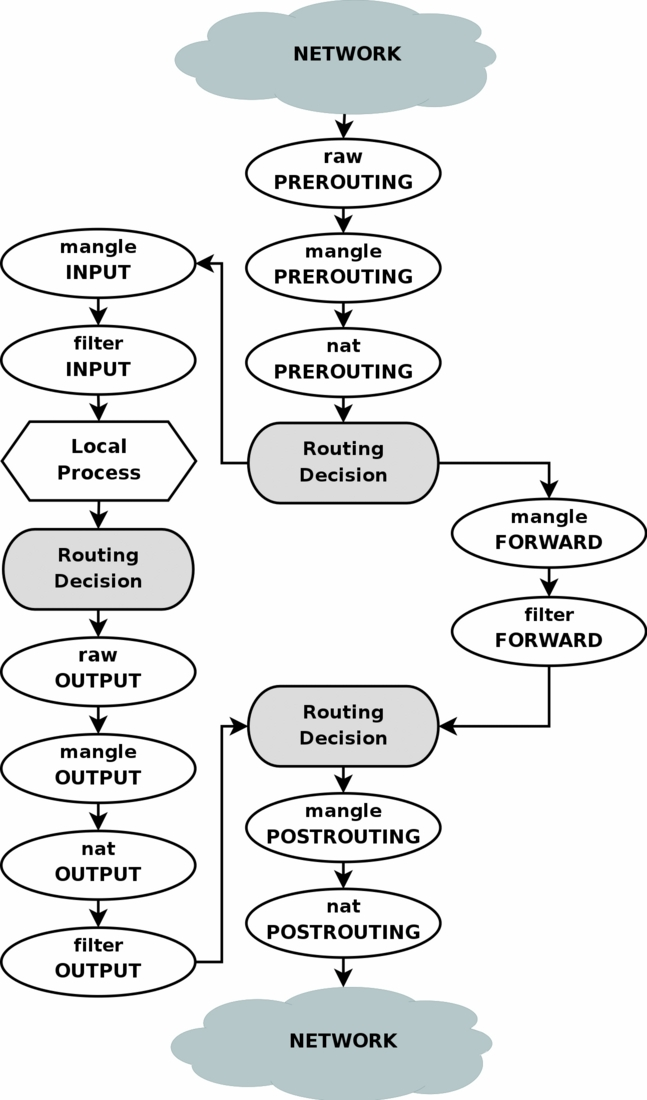
\includegraphics[width=\textwidth]{tables_traverse}
    \caption{\cite{Iptables99:online}}
\end{figure}

\section{Routing tables}
\section{Network namespaces}


\chapter{Example usecases}
pass
\section{OpenVPN on Google cloud platform}
pass
\section{Isolating process in its own network namespace}

\section{Disabling internet access for specific device at specific time}

For example you might have a really smart teen adicted to the internet.
And you'd like disabling his internet access at the router level at certain times, while keeping rest functioning. 
It can be simly done with one iptables command and few extra modules

\texttt{
    iptables -A PREROURING -m mac --mac-source 00:0F:EA:91:04:08 -m time --timestart 9:00 --timestop 18:00 -j ACCEPT\\
    iptables -A PREROURING -m mac --mac-source 00:0F:EA:91:04:08 -j DROP
}

This is more efficient than IP filtering since you're probably running DHCP on your network dynamically assigning IP addresses. 
Nevertheless, it's easy for attacker (your teen) to figure out his MAC address is filterer, and to spoof it. 
Yet, hopefully by the time he figures it out, he'll alread be a functional adult.

\bibliography{refs}
\bibliographystyle{fer}

\end{document}
